\section{EpToTester}
\label{sec:epto}
\begin{figure}[htp]
	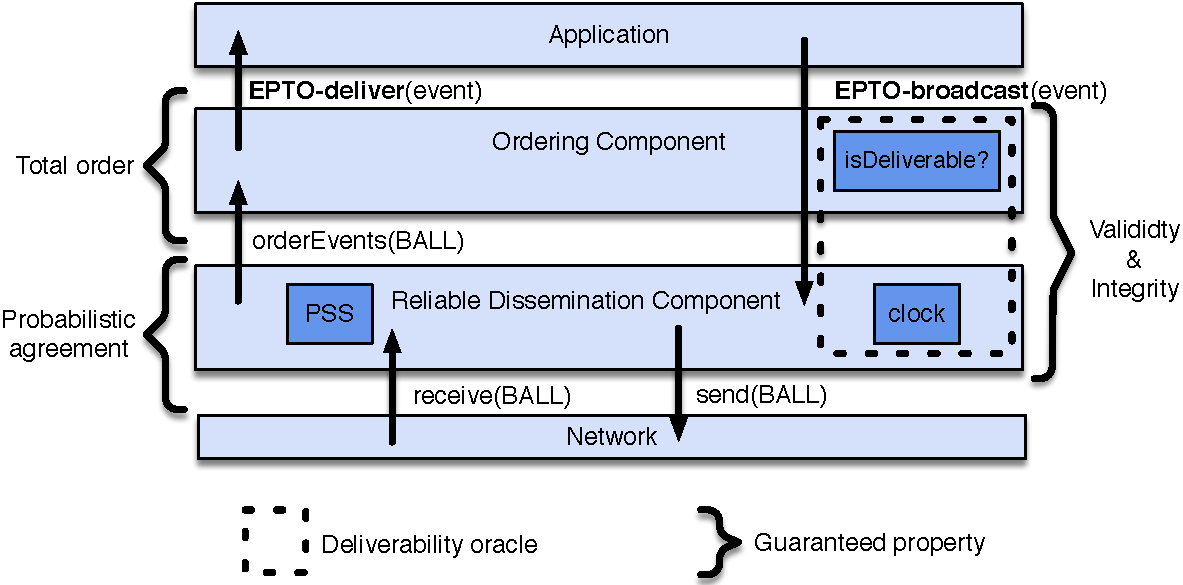
\includegraphics[width=\linewidth]{figures/architecture.pdf}
	\caption{\epto architecture \autocite{matos2015epto}.}
	\label{fig:epto-architecture}
\end{figure}
\eptotester is a practical implementation of \epto designed to assess the claims made in \autocite{matos2015epto}. Although the implementation in written with benchmarking in mind, the code could be adapted for real applications with only minimal changes to the sources. \eptotester is open-sourced on Github\footnote{\href{https://github.com/jocelynthode/EpTOTester}{https://github.com/jocelynthode/EpTOTester}}.
\subsection{Architecture}
\autoref{fig:epto-architecture} illustrates the architecture of a single replica. An application extending our Application class can \epto-broadcast and \epto-deliver events. Events broadcasted to the Dissemination component are sent over the network every $\delta$ period. Every ball received from the network is unwrapped and its events are analyzed by the Dissemination component to find out whether they need to be propagated further or not according to their Time To Live (TTL). They are then sent to the ordering component so that \epto can determine whether to deliver these events or not and in which order. The order is based on the timestamp of the events given by the logical clock and their broadcaster ID in case of a tie. The network layer communication is done using UDP and a PSS CYCLON to obtain a random view of peers. To obtain an initial random view, we contact an independent tracker that keeps track of dead and alive nodes in the system. We want to emphasize that the tracker is not required. In practice it works well, but using a DHT is certainly a possibility.
\subsection{Implementation}
We implement the payload as randomly generated UUIDs. We implement our own PSS CYCLON operating on its own port.  We compare \epto to the deterministic total order algorithm provided by \jgroups. We use \jgroups 3.6.11. When implementing \jgroups we use TCPGOSSIP provided by the \jgroups library instead of the traditional MULTICAST option to coordinate peers. This is not a problem as in a real WAN \jgroups could not rely on MULTICAST.
\subsection{Deployment}
 \begin{figure}[htp]
 	\centering
 	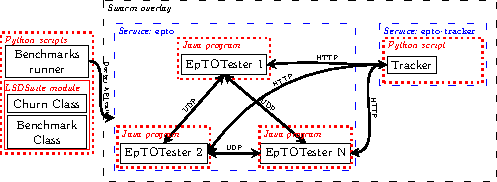
\includegraphics[width=\linewidth]{figures/complete-architecture.pdf}
 	\vspace{-2mm} 
 	\caption[Caption]{\eptotester architecture\footnotemark}
 	\vspace{-2mm} 
 	\label{fig:complete-architecture}
 \end{figure}
\footnotetext{This figure is partially inspired from a figure in \autocite{vaucher2016erasure}}
To deploy \epto effectively we need two different Docker Swarm services: one containing the tracker and one containing all \epto replicas. Both of these services use the same network overlay to communicate. This is achieved using Docker and especially the new Docker Swarm introduced in Docker 1.12. This lets us have a unified way of deploying our benchmarks locally or remotely on vastly different clusters with minimal modifications. Every benchmark is started through a Python script available on the master node. This script handles everything from starting benchmarks, scaling the cluster during a churn and collecting results. All \epto parameters are customizable by using options provided through this script.
Gradle\footnote{\href{https://gradle.org/}{https://gradle.org/}} is used to automate the project building. Finally, a script is provided to push the images to a repository accessible to the remote cluster and to push the benchmarking script on the master node. \jgroups deployment is much the same. The entire \eptotester architecture is shown in \autoref{fig:complete-architecture}.
\subsection{Fault Injection}
Our framework supports the ability to inject synthetic and real traces thanks to the work done in \autocite{vaucher2016erasure}. The synthetic churn provided by it was improved to support adding and removing nodes at the same time.
